\chapter{Recomanadors analitzats}

En aquest apartat s'explicaran les diferents proves que s'han realitzat fins a arribar al recomanador final d'aquest projecte.

\section{Avaluació del sistema}

Per tal de poder apreciar la qualitat del sistema, i la millora al realitzar diferents adicions, s'ha fet servir un sistema bastant standard en l'avaluació de recomanadors, que és el càlcul del RMSE\footnote{Root Median Square Error}. Aquest és un sistema que calcula de quant s'ha equivocat el sistema en les prediccions de les puntuacions predites a les reals. Per a això, el que fa el càlcul que es pot trobar a l'equació \ref{math-rmse-formula}.

\begin{mycapequ}[h]
\caption{Fòrmula del RMSE.}
\label{math-rmse-formula}
\begin{equation}
RMSE=\sqrt{\frac{\sum_{i=1}^{n}{(predicio_i - valor_i)}^2}{n}}
\end{equation}
\end{mycapequ}

Apart d'això, també s'ha analitzat la velocitat del sistema realitzant recomanacions, ja que apart de quan bons són els resultats que es poden obtenir d'un recomanador, també ens interesa saber si pot donar els resultats de forma ràpida.

\section{Implementació dels recomanadors}

Els recomanadors explicats a continuació han estat realitzats i avaluats mitjançant el modul Taste, de Mahout \cite{Apache-Mahout}. Aquest mòdul conté implementacions de bastants sistemes de recomanació, per tant el que s'ha hagut de fer principalment és analitzar els diferents posibles paràmetres.


\section{Recomanador basat en veïnatge}

El primer recomanador que s'ha realitzat ha estat un recomanador basat en veïnatge. Aquest recomanador es basa en buscar quan semblants són dos usuaris, per a veure quina importancia poden tenir les recomanacions d'un en les de l'altre.

\subsection{Funcionament}

La base del funcionament d'aquest recomanador resulta bastant senzilla. Consisteix en, donades les puntuacions a diferents pel·lícules per part de dos usuaris, calcular quan semblants són. Per a això, es té en compte:

\begin{itemize}
	\item Nombre de pel·lícules que comparteixen.
	\item Similitut entre les votacions en les pel·lícules compartides
\end{itemize}

Aquesta distancia es pot calcular amb diferents algoritmes. En el nostre cas, hem utilitzat la \emph{distància logarítmica}.

Un cop realitzat aquest procés per a totes les parelles d'usuaris, ja es poden realitzar recomanacions. Per a realizar una recomanació, el que es fa es una estimació de la nota que posaria l'usuari a les pel·lícules que no ha vist encara. Aquesta estimació es realitzada mirant la puntuació que han donat altres usuaris a aquestes pel·lícules, com es pot veure a l'algorisme \ref{algorithm-rating-calculation}.

\begin{algorithm}
\caption{Algoritme de predicció de la puntuació d'una pel·lícula}
\label{algorithm-rating-calculation}
\begin{algorithmic}
\State $puntuacio\_acumulada \gets 0$
\State $semblanca\_acumulada \gets 0$

\For{$puntuacio \gets pelicula\_no\_vista.puntuacions$}
	\State $un\_altre\_usuari \gets puntuacio.usuari$
	\State $semblanca \gets calcular\_semblanca(usuari, un\_altre\_usuari)$
	\State $puntuacio\_acumulada \gets puntuacio\_acumulada + puntuacio.valor \times semblanca$
	\State $semblanca\_acumulada \gets semblanca\_acumulada + semblanca$
\EndFor

\Return{$ puntuacio\_acumulada / semblanca\_acumulada$}
\end{algorithmic}
\end{algorithm}

S'ha de realitzar aquest càlcul per a cada pel·lícula i un cop fet, ordenarles en funció de la puntuació predita per tal de mostrar a l'usuari les pel·lícules que es mes probable que li interesi veure.

A la mínima que el nombre d'usuaris i pel·lícules creix, aquest càlcul resulta cada cop més pesat per al sistema, fins que resulta imposible realitzarlo. Les formes de reduir aquest calcul serien reduir el nombre de pel·lícules a contemplar o reduir el nombre d'usuaris a contemplar. Donat que de les pel·lícules no sabem encara quines li poden agradar i quines no, el mes senzill es reduir el nombre d'usuaris a tenir en compte.

Per tant, el que es fa per a reduir el nombre de càlculs a realitzar és reduir el nombre d'usuaris que es faràn servir per a predir les pel·lícules que li poden interesar a un usuari. Això es pot fer tant agafant els N usuaris més semblants com agafant tots els usuaris fins a una determinada semblança. S'ha optat per la primera opció, i s'ha acabat donant un valor prou gran com per a tenir en consideració múltiples tipus d'usuari, 100.

\subsection{Adicions al sistema}

Fins ara s'ha parlat d'utilitzar les pel·lícules que tenen en comú dos usuaris per a determinar quan semblants són. Aquesta mètrica es bona, però es pot arribar a millorar. Per a això, el que es pot fer es tenir en compte dades que es tinguin de l'usuari.

S'ha realitzat una implementació molt simple tenint en compte dades adicionals dels usuaris. Concretament, les dades que s'han tingut en compte han estat les següents:

\begin{itemize}
	\item Sexe
	\item Grup d'edat
	\item Localització
\end{itemize}

Apart de l'avantatge d'afegir noves variables al sistema, fent que, un cop entrenat correctament, pugui ser més precis, afegeix l'avantatge de tenir variables abans de que l'usuari hagi puntuat gaires pel·lícules, facilitant el funcionament del sistema per a usuaris que tenen poques pel·lícules puntuades al sistema.

\section{Slope-One}

Aques recomanador s'ha introduit a la comparació ja que es un recomanador que, tot i ser semblant a l'anterior, dona molts bons resultats.

\subsection{Funcionament}

Aquest recomanador el que fa és, donada una pèl·licula de la qual volem saber la posible puntuació per a un usuari, mirar la puntuació de pel·lícules que l'usuari comparteixi amb gent que ha vist la pel·lícula en questió. Per a això, el que es fà es calcular les diferències entre cadascuna de les pel·lícules. El que es fa a l'entrenament és calcular les diferències entre cada parella de pel·lícules, com es mostra a l'algorisme \ref{algorithm-training-slope-one}. Un cop calculades les diferencies, l'estimació de les puntuacions es realitza amb l'algorisme \ref{algorithm-recommend-slope-one} \cite{slope-one-wiki}.


\begin{algorithm}
\caption{Entrenament del Slope-One}
\label{algorithm-training-slope-one}
\begin{algorithmic}
\State $usuaris \gets usuaris\_amb\_ambudes\_pelicules(pelicula1, pelicula2)$
\State $diferencia\_puntuacions \gets 0$
\State $nombre\_puntuacions \gets comptar(usuaris)$
\For{$usuari \gets usuaris$}
	\State $diferencia\_puntuacions \gets diferencia\_puntuacions + obtenir_puntuacio(usuari, pelicula1) - obtenir_puntuacio(usuari, pelicula2)$
\EndFor
\State $diferencies[pelicula1][pelicula2] \gets diferencia\_puntuacions$
\State $pes\_diferencies[pelicula1][pelicula2] \gets diferencia\_puntuacions$

\State $diferencies[pelicula2][pelicula1] \gets - diferencia\_puntuacions$
\State $pes\_diferencies[pelicula2][pelicula1] \gets diferencia\_puntuacions$
\end{algorithmic}
\end{algorithm}

\begin{algorithm}
\caption{Recomanació del Slope-One}
\label{algorithm-recommend-slope-one}
\begin{algorithmic}
\State $puntuacions\_acumulades \gets 0$
\State $pes\_puntuacions\_acumulat \gets 0$

\For{$puntuacio \gets usuari.puntuacions$}
	\State $pelicula\_vista \gets puntuacio.pelicula$
	\State $puntuacions\_acumulades \gets puntuacions\_acumulades + (puntuacio.valor + diferencies[pelicula\_no\_vista][pelicula\_vista]) \times pes\_diferencies[pelicula\_no\_vista][pelicula\_vista]$
	\State $pes\_puntuacions\_acumulat \gets pes\_puntuacions\_acumulat + pes\_diferencies[pelicula\_no\_vista][pelicula\_vista]$
\EndFor

\Return{$puntuacions\_acumulades / pes\_puntuacions\_acumulat$}

\end{algorithmic}
\end{algorithm}

\section{Recomanador basat en la descomposició en vectors singulars}

El recomanador basat en la descomposició en vectors singulars es basa en calcular uns vectors de característiques dels usuaris i de les pel·lícules. El que fa llavors no es treballar directament amb els valors de les puntuacions a l'hora de fer les estimacions, sinó que treballa amb una estructura intermitja, bastant més compacta.

\subsection{Funcionament}

El primer que s'ha de fer es obtenir les matrius que s'han comentat de característiques d'usuaris i característiques de pel·lícules. La llibreria utilitzada ja dú varies implementacions, però únicament n'he estudiada una. El que fa aquesta implementació és, simplement, per a cada característica de cada usuari, calcular la predicció del resultat, i observant l'error, anar estimant un valor cada cop més bó per a la característica. Un cop s'han calculat aquestes matrius, per a fer la predicció d'una pel·lícula no vista per un usuari, el que s'ha de fer és simplement multiplicar el vector de característiques de l'usuari per el vector de característiques de la pel·lícula. Això fa que el nombre d'operacions per a l'estimació de la puntuació d'una pel·lícula sigui molt reduït, a a més a més, constant. Sempre s'han de realitzar tantes multiplicacions i sumes com característiques hi hagi.

\section{Resultats}

A la figura \ref{figure-rmse-scores} es pot apreciar que Slope-One i SVD funcionen molt millor que el recomanador basat en veïnatge. Aquests gràfics han estat realitzats executant l'algorisme del RMSE deu vegades per a cada procés. S'ha realitzat una segona execució, de 20 iteracions i més variacions d'aquests 2 algorismes. Els resultats es poden apreciar a la figura \ref{figure-rmse-scores-specific}.

Un altre element que s'ha estudiat es la velocitat amb la que els diferents sistemes calculen les recomanacions, ja que és un punt que resulta bastant interesant per a la recomanació web. A la figura \ref{figure-recommender-speed} es pot veure una comparativa dels diferents sitemes. A aquest gràfic es pot apreciar que els càlculs realitzats són molt més ràpids a Slope-One i a SVD. Aquest últim té uns temps de càlcul molt baixos ja que el nombre d'operacions a realitzar per a cada estimació és molt reduit.

\begin{figure}[h!]
  \caption{RMSE dels diferents algorismes.}
  \label{figure-rmse-scores}
  \centering
    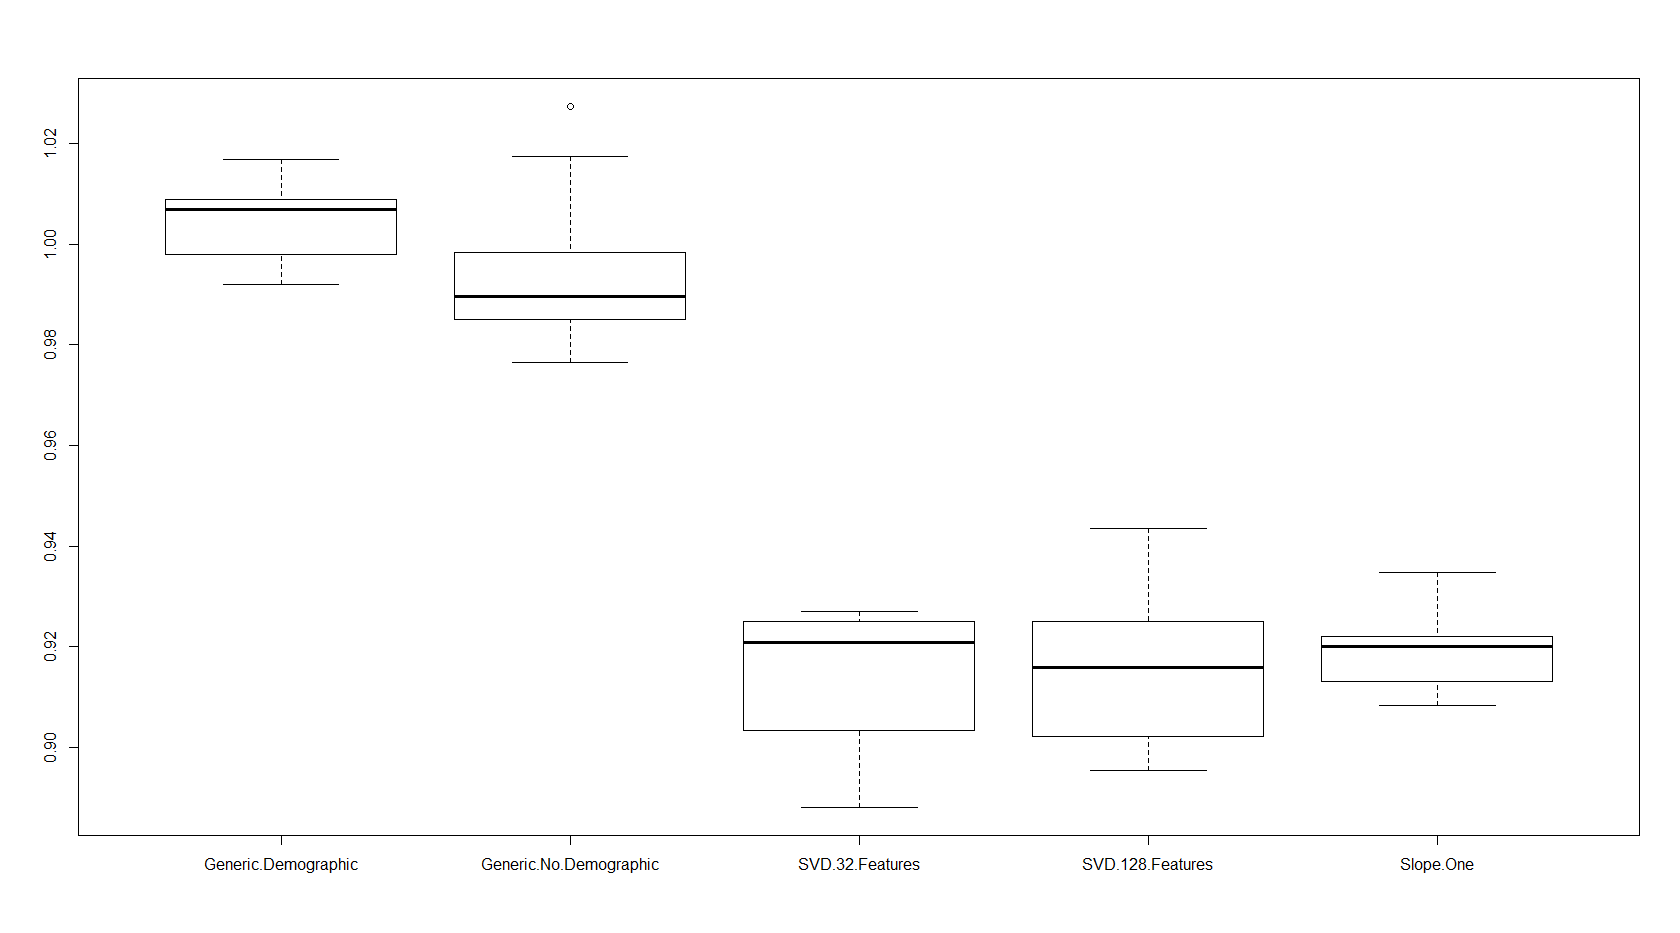
\includegraphics[width=\textwidth]{figs/resultats_10iter.png}
\end{figure}

\begin{figure}[h!]
  \caption{RMSE de diferents variants del SVD i Slope-One.}
  \label{figure-rmse-scores-specific}
  \centering
    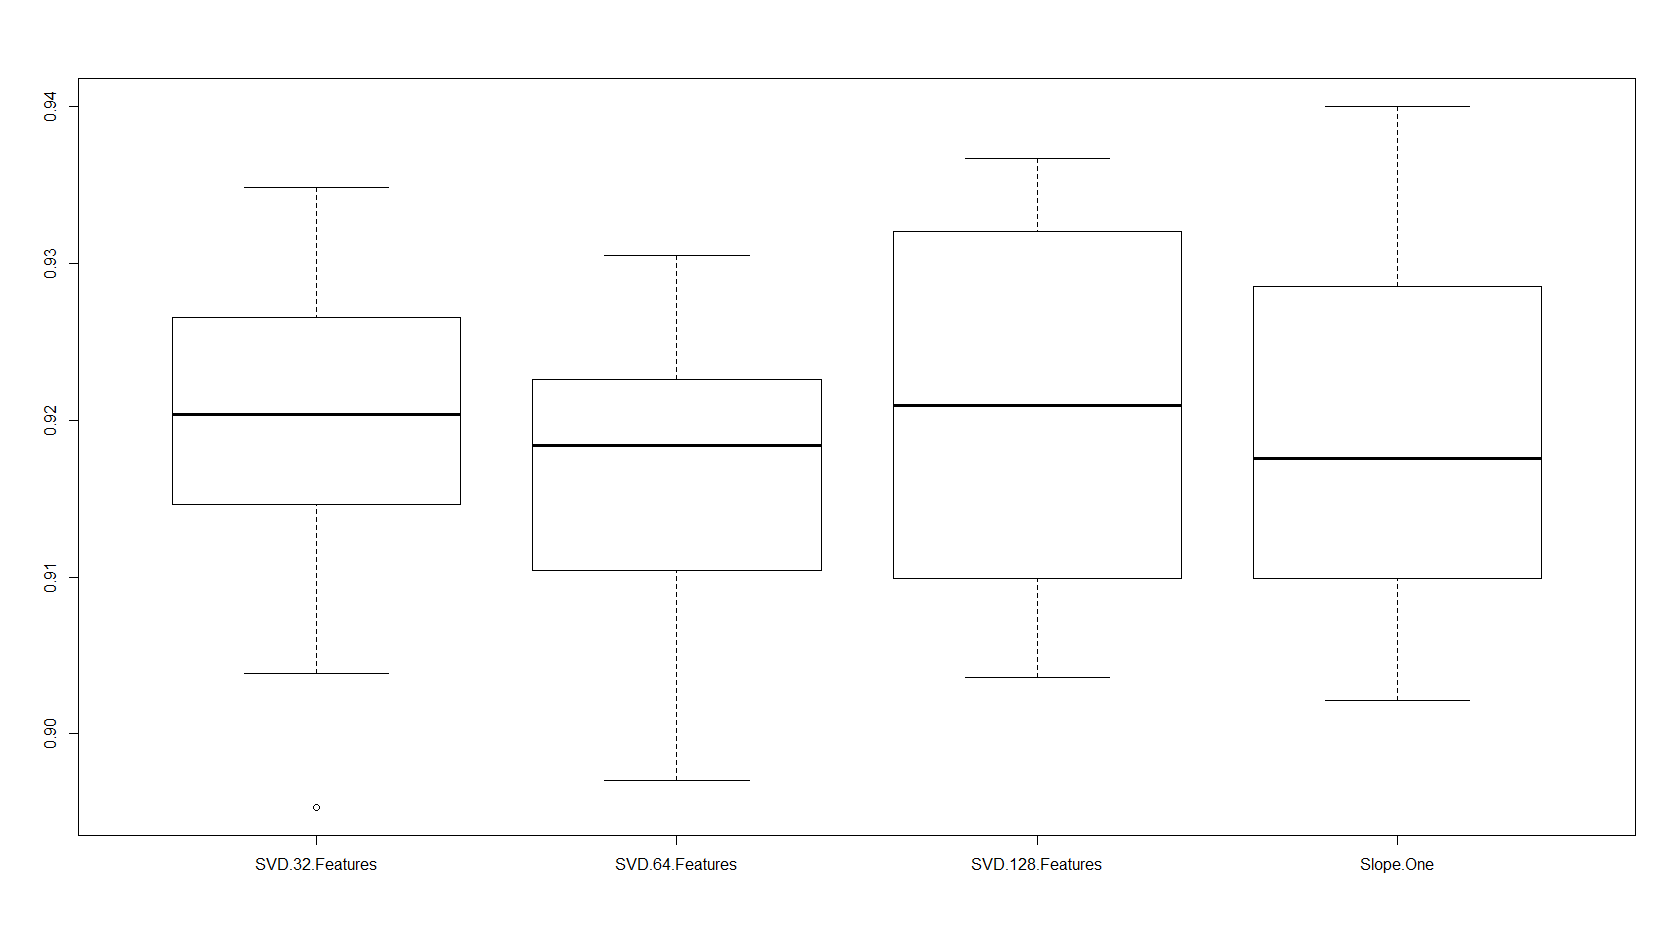
\includegraphics[width=\textwidth]{figs/resultats_20iter_specific.png}
\end{figure}

\begin{figure}[h!]
  \caption{Temps tardat en realitzar recomanacions pels diferents sistemes.}
  \label{figure-recommender-speed}
  \centering
    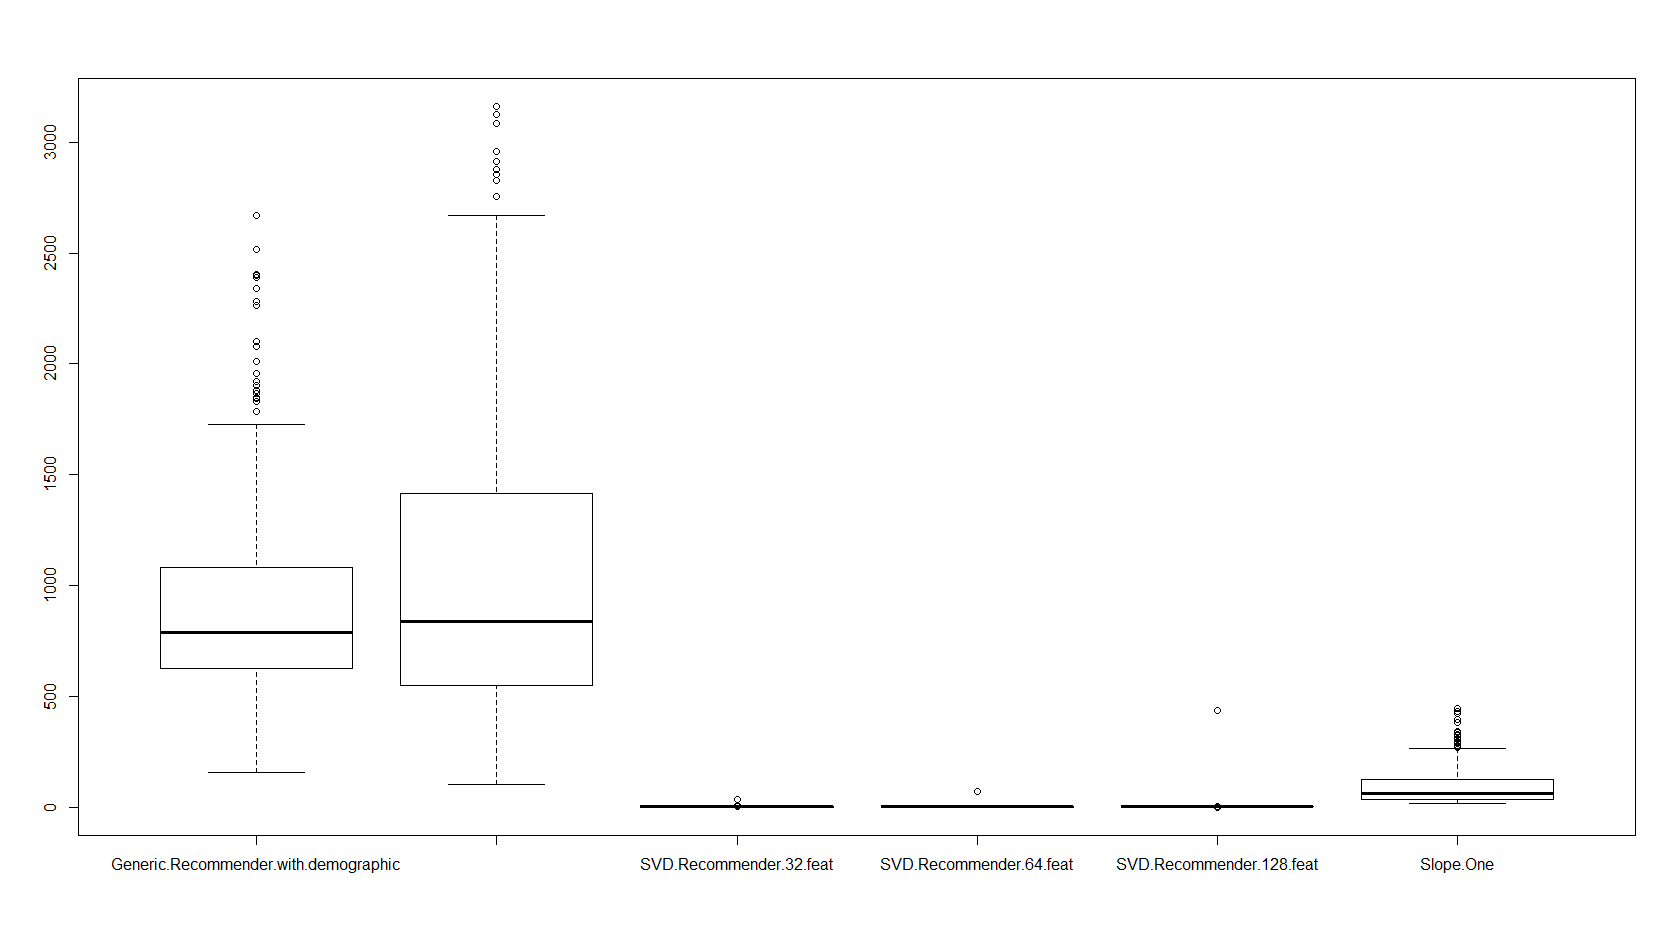
\includegraphics[width=\textwidth]{figs/times.png}
\end{figure}

Donats aquests resultats, el recomanador que anirà millor per a la web seria el SVD, ja que dona bons resultats, i a més a més, és el sistema més ràpid amb bastanta diferència.
